\title{Neuron}
\date{}

\documentclass[12pt]{article}

\usepackage[italian]{babel}
\usepackage[T1]{fontenc}
\usepackage[utf8]{inputenc}
\usepackage{graphicx}
\usepackage{amsmath}
\usepackage{amssymb}
\usepackage{float}

\begin{document}
\maketitle
\newpage

\section{Introduzione}
In questa relazione si illustrerà l'implementazione di un singolo neurone artificiale, il quale verrà adattato in modo da interpolare le funzioni logiche \emph{AND} e \emph{OR}, mediante l'utilizzo dell'\emph{Hebbian learning}.

\section {Neurone artificiale}
Un neurone artificiale è un oggetto matematico con $N$ ingressi e un uscita, l'uscita del neurone è valutata mediante il passaggio degli ingressi attraverso due stadi. Il primo stadio, lineare, è calcolata mediante la combinazione lineare tra gli $N$ ingressi ($x_i$) e un insieme di $N$ pesi ($w_i$). Si usa predisporre un peso aggiuntivo ($w_0$) che fa da \emph{bias} e impone il valore medio dell'output lineare. L'uscita dello stadio lineare del neurone viene infine valutata da una funzione non lineare detta \emph{di attivazione} la quale usualmente è un \emph{gradino} o una sua approssimazione derivabile, come ad esempio una \emph{sigmoide}.

\begin{figure}[h]
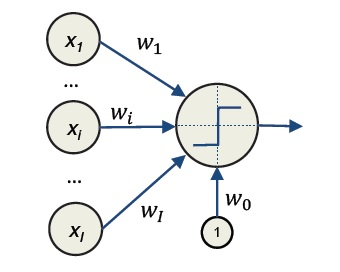
\includegraphics{Neuron.jpg}
\centering
\end{figure}

L'uscita del neurone è quindi esprimibile nella seguente forma:
$$ h_j (x | w,b) = h_j \bigg( \sum_{i=1}^{N} w_i \cdot x_i - b \bigg) = h_j \bigg( \sum_{i=0}^{N} w_i \cdot x_i \bigg) = h_j \mathbf{w^T x} $$

Dove $x$ sono gli ingressi e $w$ i pesi.

\subsection{Hebbian learning}
L'Hebbian learning è stato il primo algoritmo di \emph{learning} del singolo neurone artificiale.

Si sceglie un \emph{learning rate} $ \eta $ e si aggiornano i pesi del neurone mediante una semplice procedura di aggiornamento dello stato:
$$ w_{i}^{\langle k+1 \rangle} = w_i^{\langle k \rangle} + \eta \cdot x_i^{ \langle k \rangle} \cdot t^{ \langle k \rangle } $$

Dove $x_i^{ \langle k \rangle}$ è l'ingresso all'istante \emph{k-esimo} e $t^{\langle k \rangle}$ l'uscita desiderata al medesimo istante. Si itera finchè il risultato in uscita dal neurone non è  uguale a quello desiderato.

Nella computazione delle due funzioni logiche è stato utilizzato l'Hebbian learning, tuttavia per interpolare funzioni più complesse sarebbe stato necessario utilizzare le migliori tecniche di \emph{back propagation}.

\section{Risultati}
Il risultato del learning per le due funzioni è il seguente:

$$
\mathbf{w_{OR}^T} = 
\begin{bmatrix}
-3  &    1.51 &  1.51 \\
\end{bmatrix}
$$
$$
\mathbf{w_{AND}^T} = 
\begin{bmatrix}
0   &    0.01 &   0.01 \\
\end{bmatrix}
$$
e permettono di eseguire correttamente il calcolo.


\end{document}
